\documentclass{beamer}
 
\usepackage[utf8]{inputenc}
\usetheme{Copenhagen}
\usepackage{minted}
\usepackage{listings,xcolor}
\usepackage{xcolor}

\lstdefinelanguage{elixir}{
    morekeywords={case,catch,def,do,else,false,%
        use,alias,receive,timeout,defmacro,defp,%
        for,if,import,defmodule,defprotocol,%
        nil,defmacrop,defoverridable,defimpl,%
        super,fn,raise,true,try,end,with,%
        unless},
    otherkeywords={<-,->, |>, \%\{, \}, \{, \, (, )},
    sensitive=true,
    morecomment=[l]{\#},
    morecomment=[n]{/*}{*/},
    morecomment=[s][\color{purple}]{:}{\ },
    morestring=[s][\color{orange}]"",
    commentstyle=\color{commentgreen},
    keywordstyle=\color{eminence},
    stringstyle=\color{red},
	basicstyle=\ttfamily,
	breaklines,
	showstringspaces=false,
	frame=tb
}

\defverbatim[colored]\CustomScalarType{
  \begin{lstlisting}[language=elixir, caption={Custom Scaler Type}, captionpos=b, basicstyle=\footnotesize, numbers=left]
  scalar :date do
    parse(fn input ->
      case Timex.parse!(input.value, "{YYYY}-{0M}-{D}") |> DateTime.from_naive("Etc/UTC") do
        {:ok, date} -> {:ok, date}
        _ -> :error
      end
    end)

    serialize(fn date -> Date.to_iso8601(date) end)
  end
  \end{lstlisting}
}

\defverbatim[colored]\EnumType{
  \begin{lstlisting}[language=elixir, caption={Enum Type}, captionpos=b, basicstyle=\scriptsize, numbers=left]
    enum :priority_level, description: "Todo priority levels" do
      value :high, as: :true, description: "High Priority"
      value :low, as: :false, description: "Low Priority"
    end
  \end{lstlisting}
}

%Information to be included in the title page:
\title{Server Side GraphQL}
\subtitle{Using Elixir, Phoenix and Absinthe}

\author[rlb3]{Robert Boone}
\institute[C1]{ChaiOne}
\date{June 27, 2018}
\logo{
\includegraphics[height=1.0cm]{absinthe-logo}} 
 
 
\begin{document}
 
\frame{\titlepage}

\begin{frame}
\frametitle{Table of Contents}
\tableofcontents
\end{frame}

\section{Introduction}

\begin{frame}
\frametitle{What is GraphQL?}
GraphQL is a data \alert{query language} developed by Facebook in 2012 and release in 2015.
\end{frame}

\begin{frame}
  \frametitle{Query Language}

  \begin{itemize}
    \item{A language for the specification of procedures for the retrieval (and sometimes also modification) of information from a database.} \pause

    \item{The fact that GraphQL can be used as a web API is an implementation detail.}

  \pause

  \item{It's has more in common with SQL than it does with REST.}
  \end{itemize}

\end{frame}

\section{Fundamentals}

\begin{frame}
  \frametitle{Types}

  APIs in GraphQL are organized by types and fields.
  \begin{block}{Builtin Types}
    \begin{itemize}
    \item{boolean}
    \item{float}
    \item{id}
    \item{integer}
    \item{string}
    \end{itemize}
  \end{block}
\end{frame}

\begin{frame}
  \frametitle{Types}
  You can also create custom Scalar Types.

  \CustomScalarType
\end{frame}

\begin{frame}
  \frametitle{Types}
  ... Enum Types
  \EnumType

\end{frame}

\begin{frame}
  \begin{center}
    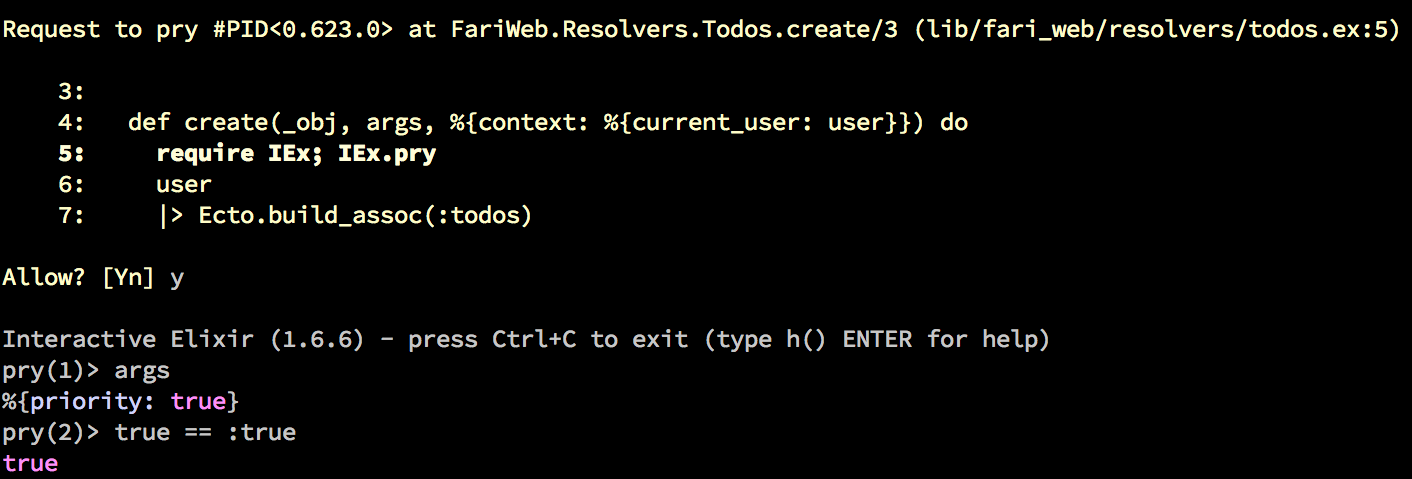
\includegraphics[width=1\paperwidth]{enum_example}
  \end{center}
\end{frame}

\section{Building A Server}

\end{document}

